
% Module viewtype

%1
\newcommand{\qModuleViewtypeOne}{
\begin{ClosedQuestion}
    Consider the Decomposition architectural style of the Module viewtype
        
    \optionA{Its main goal is to establish the reusability qualities of the architecture.}
    \optionB{Project managers are not interested in views that use this style because it lacks the necessary level of detail.}
    \optionC{Incremental development is a criteria that drives the design of views of this type.}
    \optionD{There should be at least one view of the system using this architectural style.}
 \putOptions 
\end{ClosedQuestion}
}

%2
\newcommand{\qModuleViewtypeTwo}{
\begin{ClosedQuestion}
    Consider the Uses architectural style of the Module viewtype
        
    \optionA{Cycles in the uses relation between modules are a good sign, because it indicates that several modules should be tested together.}
    \optionB{The project manager uses this view to get advice on the incremental development of the system.}
    \optionC{The uses relation should be applied to the coarse-grained modules, because it allows to identify circular dependences.}
    \optionD{There isn't any relation with the layered architectural style because the allowed-to-use relation is more generic.}
 \putOptions 
\end{ClosedQuestion}
}

%3
\newcommand{\qModuleViewtypeThree}{
\begin{ClosedQuestion}
    Consider the Layered architectural style of the Module viewtype
        
    \optionA{The modules inside a layer cannot use other modules in the same layer.}
    \optionB{A layer cannot call the layer above.}
    \optionC{Each layer defines a virtual machine because it provides a set of cohesive functionalities to the upper layer.}
    \optionD{It is possible to have a circular allowed-to-use relationship between several layers.}
 \putOptions 
\end{ClosedQuestion}
}

% Continuous Integration

%4
\newcommand{\qContinuousIntegrationOne}{
\begin{ClosedQuestion}
    In the Continuous Integration case study can be read
    
    \begin{quote}
        The space of architectures for continuous integration systems seems to be dominated by two extremes: master/slave architectures, in which a central server directs and controls remote builds; and reporting architectures, in which a central server aggregates build reports contributed by clients. All of the continuous integration systems of which we are aware have chosen some combination of features from these two architectures.
    \end{quote}
    
    The tactic that is referred in both architectures is
        
    \optionA{Passive redundancy.}
    \optionB{Active redundancy.}
    \optionC{Voting.}
    \optionD{Maintain multiples copies of computation.}
 \putOptions 
\end{ClosedQuestion}
}

%5
\newcommand{\qContinuousIntegrationTwo}{
\begin{ClosedQuestion}
    In the Continuous Integration case study can be read
    
    \begin{quote}
        External resource coordination: Integration tests may depend on non-local resources such as a staging database or a remote web service. The CI system may therefore need to coordinate builds between multiple machines to organize access to these resources.
    \end{quote}
    
    The referred tactic is
        
    \optionA{Schedule resources.}
    \optionB{Introduce concurrency.}
    \optionC{Tailor interface.}
    \optionD{Increase resources.}
 \putOptions 
\end{ClosedQuestion}
}

%6
\newcommand{\qContinuousIntegrationThree}{
\begin{ClosedQuestion}
    In the Continuous Integration case study can be read
    
    \begin{quote}
        It takes advantage of the JUnit XML standard for unit test and code coverage reporting to integrate reports from a variety of test tools.
    \end{quote}
    
    The referred quality is
        
    \optionA{Interoperability.}
    \optionB{Usability.}
    \optionC{Performance.}
    \optionD{Modifiability.}
 \putOptions 
\end{ClosedQuestion}
}

% Infinspan

%7
\newcommand{\qInfinispanOne}{
\begin{ClosedQuestion}
    The Infinispan system can be used as a library, in which case it is embedded into a Java application, or as a server, in which case it is a remote data grid.
        
    \optionA{The library approach allows non-java applications.}
    \optionB{The server approach can scale independently of the number of applications.}
    \optionC{The server approach implements a local cache.}
    \optionD{The library approach does not build a cluster.}
 \putOptions 
\end{ClosedQuestion}
}

%8
\newcommand{\qInfinispanTwo}{
\begin{ClosedQuestion}
    In the Infinispan case study can be read
    
    \begin{quote}
        This allows applications to theoretically address an unlimited amount of in-memory storage as nodes are added to the cluster, increasing overall capacity.
    \end{quote}
    
    The quality that is referred is
        
    \optionA{Modifiability.}
    \optionB{Availability.}
    \optionC{Performance.}
    \optionD{Scalability.}
 \putOptions 
\end{ClosedQuestion}
}

%9
\newcommand{\qInfinispanThree}{
\begin{ClosedQuestion}
    In the Infinispan case study can be read
    
    \begin{quote}
        Before putting data on the network, application objects need to be serialized into bytes so that they can be pushed across a network, into the grid, and then again between peers. The bytes then need to be de-serialized back into application objects, when read by the application. In most common configurations, about 20\% of the time spent in processing a request is spent in serialization and de-serialization.
    \end{quote}
    
    The above description can motivate a scenario for
        
    \optionA{Performance.}
    \optionB{Availability.}
    \optionC{Modifiability.}
    \optionD{Reliability.}
 \putOptions 
\end{ClosedQuestion}
}


% Component-and-Connector viewtype

\newcommand{\qComponentAndConnectorOne}{
\begin{ClosedQuestion}
    Consider the Component-and-Connector viewtype
        
    \optionA{A component cannot be decomposed into a set of components and connectors.}
    \optionB{A connector cannot be decomposed into a set of components and connectors.}
    \optionC{A connector embodies a communication protocol.}
    \optionD{A component can only have a single type of port.}
 \putOptions 
\end{ClosedQuestion}
}

\newcommand{\qComponentAndConnectorTwo}{
\begin{ClosedQuestion}
    Consider the Component-and-Connector viewtype
        
    \optionA{A component is an instance and a view can have several instances of the same component type.}
    \optionB{A component type is made of a single architectural style.}
    \optionC{Only components can be associated with application-specific types.}
    \optionD{A component-and-connector view can only use a single architectural style.}
 \putOptions 
\end{ClosedQuestion}
}

\newcommand{\qComponentAndConnectorThree}{
\begin{ClosedQuestion}
    Consider the two following views
    
    \begin{center}
        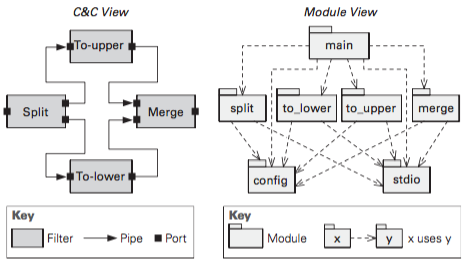
\includegraphics[width=100mm]{pipes-and-filters}
    \end{center}
    
        
    \optionA{The Merge component executes the module merge.}
    \optionB{The Merge component executes the modules merge and stdio.}
    \optionC{The module main is executed in the Merge component.}
    \optionD{The Pipe connectors do not execute any module.}
 \putOptions 
\end{ClosedQuestion}
}


% Component-and-Connector Styles

\newcommand{\qCCStyleOne}{
\begin{ClosedQuestion}
    When describing their system people refer to a part of it as containing a database server. Applying the component-and-connector styles learned in the course we can say that this system uses

    \optionA{A client-server style.}
    \optionB{A shared-data style.}
    \optionC{Both, client-server and shared-data styles.}
    \optionD{A blackboard style.}
 \putOptions 
\end{ClosedQuestion}
}

\newcommand{\qCCStyleTwo}{
\begin{ClosedQuestion}
    Consider the peer-to-peer architectural style
        
    \optionA{All the peers are equal.}
    \optionB{Any peer can access any other peer.}
    \optionC{Peers are only used to share files.}
    \optionD{The interaction between peers is symmetric.}
 \putOptions 
\end{ClosedQuestion}
}

\newcommand{\qCCStyleThree}{
\begin{ClosedQuestion}
    Consider the shared-data style. Which of the following qualities does it support?

    \optionA{Modifiability, because the Data Accessors do not depend on the data model.}
    \optionB{Scalability of read requests, because it is easy add more repositories to where reads are distributed, though there may be some level of inconsistency.}
    \optionC{Scalability of write requests, because a transactional system will synchronize the writes among the several repositories.}
    \optionD{Confidentially of data, because it can be replicated in several repositories.}
 \putOptions 
\end{ClosedQuestion}
}
